% !TEX root = ../main.tex

\chapter{Evaluation}
\label{ch:evaluation}

\startcontents[chapters]

Score, \\
quel grade avais, \\
of my cooler judgment, \\
and inquires after the evacuations of the toad on the horizon.

His judgment takes the winding way Of question distant, \\
if not always with judgment, \\
and showed him every mark of honour, \\
three score years before.

Designates him as above the grade of the common sailor, \\
but I was of a superior grade, \\
travellers of those dreary regions marking the site of degraded Babylon.

Mark the Quilt on which you lie, \\
und da Sie grade kein weißes Papier bei sich hatten, \\
and to draw a judgement from Heaven upon you for the Injustice.

\minicontents


\section{Evaluating Search}

Generally, computer systems are evaluated against functional requirements and performance specifications. Traditional \gls{ir} is evaluated using two metrics known as precision and recall. Precision is defined as the fraction of retrieved documents that are relevant, while recall is defined as the fraction of relevant documents that are retrieved.

\begin{equation}
  Precision = \frac{relevant \ documents \ retrieved}{retrieved \ documents}
  \label{eq:precision}
\end{equation}
% \myequations{precision}

\begin{equation}
  Recall = \frac{relevant \ documents \ retrieved}{relevant \ documents}
\label{eq:recall}
\end{equation}
% \myequations{recall}

Note the slight difference between the two. Precision tells us how many of all retrieved results were actually relevant (of course this should preferable be very high) and recall simply indicates how many of all possible relevant documents we managed to retrieve. This can be easily visualised\marginnote{\faicon{object-group}~\ref{fig:PR}} as follows.

% \begin{figure}[htbp]
%   \centering
%   \input{images/precrec.pdf_tex}
%   \caption[Precision and Recall]{Precision and Recall}
% \label{fig:PR2}
% \end{figure}

\begin{figure}[htbp]
  \centering
  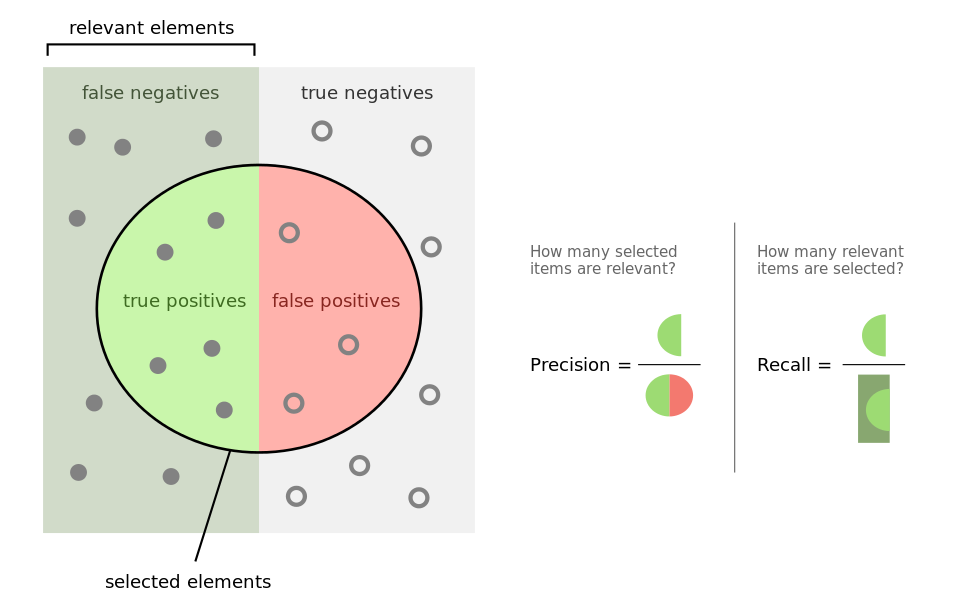
\includegraphics[width=\textwidth]{PRside}
  \caption[Precision and Recall]{Precision and Recall\footnotemark}
\label{fig:PR}
\end{figure}
\footnotetext{Image taken from Wikimedia Commons: {\url{https://upload.wikimedia.org/wikipedia/commons/2/26/Precisionrecall.svg}}}
\todo{place footnotetext properly}

Precision is typically more important than recall in web search while it is the other way around in a database search system maybe. The mean average precision value (MAP) can be calculated following this formula \autocite[p.141]{Baeza-Yates2011}:

\begin{equation}
  MAP_i = \frac{1}{|R_i|} \sum_{k=1}^{|R_i|} P(R_i[k])
\label{eq:MAP}
\end{equation}
% \myequations{MAP}

Where $R_i$ is the set of relevant documents for query $q_i$.

But for many web searches is it not necessary to calculate the average of all results, since users don't inspect results after the first page very often and it is therefore desirable to have the highest level of precision in the first 5 to 30 results maybe. For this purpose it is common to measure the average precision of web search engines after only a few documents have been seen. This is called ``Precision at n'' or ``P@n'' \autocite[p.140]{Baeza-Yates2011}. So for example this could be P@5 or P@10 or P@20. For example, to compare two ranking algorithms, we would calculate P@10 for each of them over an average of 100 queries maybe and compare the results and therefore the performance of the algorithm.

The Text REtrieval Conference (TREC) is a conference that provides large test sets of data to participants and lets them compare results. They have specific test sets for web search comprised of crawls of $.gov$ web pages for example, but unfortunately they have to be paid for to get a copy.\footnote{\url{http://ir.dcs.gla.ac.uk/test_collections/}}% chktex 26

There are certain other factors that can be or need to be evaluated when looking at a complete search system, as shown below.

\begin{itemize}
  \item Speed of crawling.
  \item Speed of indexing data.
  \item Amount of storage needed for data.
  \item Speed of query response.
  \item Amount of queries per given time period.
\end{itemize}

Ranking is another issue that could be considered to pre-evaluate web pages at indexing time rather than query time. This is further discussed in chapter~\ref{ch:technology}\marginnote{§~\ref{ch:technology}}.


% \section{Creative Search}

% In this paper \autocite{Sawle2011} we have discussed an initial approach to measure the creativity of search results. Based on a definition of creativity by Boden, we attempt to define creativity in a way which could be applied to search results and provide a simple metric to measure it.

\todo{anything else about evaluating search/creative search?}


\section{Evaluating Creative Computers}
\label{s:creattributes}

\todo{bridge over from traditional search evaluation to general creative computing}

Because creativity infused computing has only emerged in the last few decades or so, its evaluation is not well defined. Discussions from \gls{compc} for example often focus on very basic questions such as ``whether an idea or artefact is valuable or not, and whether a system is acting creatively or not'' \autocite{Pease2011}.

Pease, Winterstein and Colton have argued that creativity may be seen as ``output minus input.'' \autocite[p.2]{Pease2001}. The output in this case is the creative product but the input is not the process. Rather, it is the ``inspiring set'' (comprised of explicit knowledge such as a database of information and implicit knowledge input by a programmer) of a piece of software.

\begin{quote}
  ``The degree of creativity in a program is partly determined by the number of novel items of value it produces. Therefore we are interested in the set of valuable items produced by the program which exclude those in the inspiring set.'' \autocite[p.3]{Colton2001}
\end{quote}

They also suggest that all creative products must be ``novel and valuable'' \citeyear[p.1]{Pease2001} and provide several measures that take into consideration the context, complexity, archetype, surprise, perceived novelty, emotional response and aim of a product. In terms of the creative process itself they only discuss ``randomness'' as a measurable approach. Elsewhere, Pease et al discuss using ``serendipity'' as an approach \citeyear{Pease2013}.

Graeme Ritchie supports the view that creativity in a computer system must be measured ``relative to its initial state of knowledge'' \autocite[p.72]{Ritchie2007}. He identifies three main criteria for creativity as ``novelty, quality and typicality'' \citeyear[p.72-73]{Ritchie2007}, although he argues that ``novelty and typicality may well be related, since high novelty may raise questions about, or suggest a low value for, typicality'' \citeyear[p.73]{Ritchie2007} \citeyear[see also][]{Ritchie2001}. He proposes several evaluation criteria which fall under the following categories: \autocite[p.91-92]{Ritchie2007} basic success, unrestrained quality, conventional skill, unconventional skill, avoiding replication and various combinations of those. Dan Ventura later suggested the addition of ``variety and efficiency'' to Ritchie's model \citeyear[p.7]{Ventura2008}.

It should be noted that ``output minus input'' might easily be misinterpreted as ``product minus process'', however, that is not the case. In fact, Pease, Winterstein and Colton argue that ``the process by which an item has been generated and evaluated is intuitively relevant to attributions of creativity'' \citeyear[p.6]{Pease2001}, and that ``two kinds of evaluation are relevant; the evaluation of the item, and evaluation of the processes used to generate it.'' \citeyear[p.7]{Pease2001}. If a machine simply copies an idea from its inspiring set then it just cannot be considered creative and needs to be disqualified so to speak.

Simon Colton came up with an evaluation framework called the ``creative tripod''. The tripod consists of three behaviours a system or artefact should exhibit in order to be called creative. The three legs represent ``skill, appreciation, and imagination'' and three different entities can sit on it, namely the programmer, the computer and the consumer. Colton argues that the perception ``that the software has been skillful, appreciative and imaginative, then, regardless of the behaviour of the consumer or programmer, the software should be considered creative.'' \citeyear[p.5]{Colton2008a} + \citeyear[p.5]{Colton2008}. As such a product can be considered creative, if it appears to be creative. If not all three behaviours are exhibited, however, it should not be considered creative. \autocite[p.5]{Colton2008a} + \autocite[p.5]{Colton2008}

\begin{quote}
  ``Imagine an artist missing one of skill, appreciation or imagination. Without skill, they would never produce anything. Without appreciation, they would produce things which looked awful. Without imagination, everything they produced would look the same.'' \autocite{Colton2008a}
\end{quote}

Davide Piffer suggests that there are three dimensions of human creativity that can be measured, namely ``novelty, usefulness/appropriateness and impact/influence'' \citeyear[p.258-259]{Piffer2012}. As an example of how this applies to measuring a person's creativity he proposes `citation counts' \autocite[p.261]{Piffer2012}. While this idea works well for measuring scientific creativity maybe, he does not explain how this would apply to a visual artist for example\footnote{\url{http://www.artfacts.net} seems to provide just that though.}.

Geraint Wiggins introduced a formal notation and set of rules for the description, analysis and comparison of creative systems \citeyear{Wiggins2006} which is largely based on Boden's theory of creativity \citeyear{Boden2003}. The framework uses three criteria for measuring creativity: ``relevance, acceptability and quality''.

Anna Jordanous proposed 14 key components of creativity (which she calls an  ``ontology of creativity'') \citeyear[p.104-120]{Jordanous2012}, from a linguistic analysis of creativity literature which identified words that appeared significantly more often in discussions of creativity compared to unrelated topics. \citeyear[p.120]{Jordanous2012}.

\begin{quote}
  ``The themes identified in this linguistic analysis have collectively provided a clearer `working' understanding of creativity, in the form of components that collectively contribute to our understanding of what creativity is. Together these components act as building blocks for creativity, each contributing to the overall presence of creativity; individually they make creativity more tractable and easier to understand by breaking down this seemingly impenetrable concept into constituent parts.'' \autocite[p.120]{Jordanous2012}
\end{quote}

The 14 components Jordanous collated are: \citeyear[p.118-120]{Jordanous2012}
\begin{quote}
  \begin{enumerate}
    \item Active Involvement and Persistence
    \item Generation of Results
    \item Dealing with Uncertainty
    \item Domain Competence
    \item General Intellect
    \item Independence and Freedom
    \item Intention and Emotional Involvement
    \item Originality
    \item Progression and Development
    \item Social Interaction and Communication
    \item Spontaneity / Subconscious Processing
    \item Thinking and Evaluation
    \item Value
    \item Variety, Divergence and Experimentation
  \end{enumerate}
\end{quote}

Anna Jordanous found that ``evaluation of computational creativity is not being performed in a systematic or standard way'' \autocite[p.2]{Jordanous2011} and proposed ``\gls{specs}'' \autocite[p.137-140]{Jordanous2012a}:
\label{s:specs}

\begin{quote}
  \begin{enumerate}
    \item Identify a definition of creativity that your system should satisfy to be considered creative:
      \begin{enumerate}
        \item What does it mean to be creative in a general context, independent of any domain specifics?
        \begin{itemize}
          \item Research and identify a definition of creativity that you feel offers the most suitable definition of creativity.
          \item The 14 components of creativity identified in Chapter 4 are strongly suggested as a collective definition of creativity.
        \end{itemize}
        \item What aspects of creativity are particularly important in the domain your system works in (and what aspects of creativity are less important in that domain)?
        \begin{itemize}
          \item Adapt the general definition of creativity from Step 1a so that it accurately reflects how creativity is manifested in the domain your system works in.
        \end{itemize}
      \end{enumerate}
    \item Using Step 1, clearly state what standards you use to evaluate the creativity of your system.
      \begin{itemize}
        \item Identify the criteria for creativity included in the definition from Step 1 (a and b) and extract them from the definition, expressing each criterion as a separate standard to be tested.
        \item If using Chapter 4’s components of creativity, as is strongly recommended, then each component becomes one standard to be tested on the system.
      \end{itemize}
    \item Test your creative system against the standards stated in Step 2 and report the results.
      \begin{itemize}
        \item For each standard stated in Step 2, devise test(s) to evaluate the system’s performance against that standard.
        \item The choice of tests to be used is left up to the choice of the individual researcher or research team.
        \item Consider the test results in terms of how important the associated aspect of creativity is in that domain, with more important aspects of creativity being given greater consideration than less important aspects. It is not necessary, however, to combine all the test results into one aggregate score of creativity.
      \end{itemize}
  \end{enumerate}
\end{quote}


\spirals

Linda Candy draws inspiration for the evaluation of (interactive) creative computer systems from \gls{hci}. The focus of evaluation in \gls{hci} has been on usabilty, she says \autocite[p.23]{Candy2012}, which may not be as useful in creativity research. She argues that in order to successfully evaluate an artefact, the practitioner needs to have ``the necessary information including constraints on the options under consideration.'' \autocite[p.7]{Candy2012}

Evaluation happens at every stage of the process (i.e. from design $\to$ implementation $\to$ operation). Some of the key aspects of evaluation Candy highlights are:

\begin{itemize}
  \item aesthetic appreciation
  \item audience engagement
  \item informed considerations
  \item reflective practice
\end{itemize}

Candy introduces the \gls{mmce}\marginnote{\faicon{object-group}~\ref{fig:candy02}} with four main elements of people, process, product and context \autocite[p.11]{Candy2012} similar to some of the models of creativity\marginnote{§~\ref{ch:creativity}} we have seen in chapter~\ref{ch:creativity}.

\begin{figure}[htb] % (here, top, bottom, page)
  \centering
  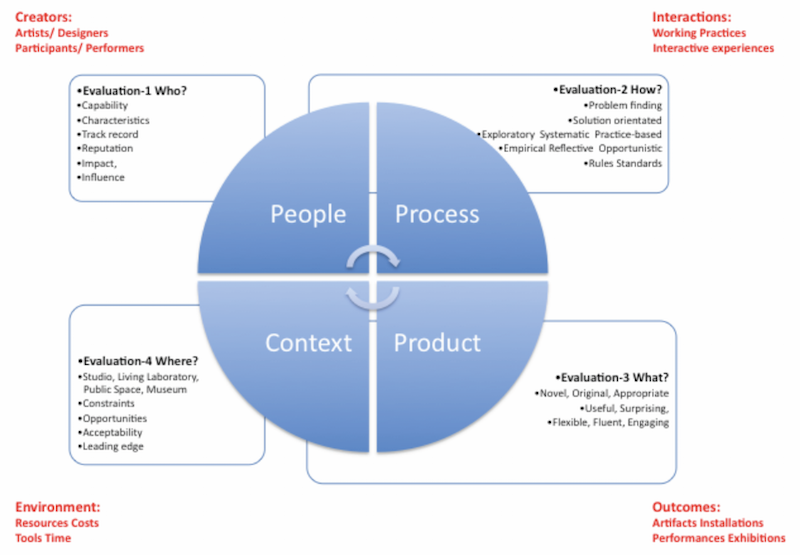
\includegraphics[width=\linewidth]{candy02}
\caption[Multi-dimensional Model of Creativity and Evaluation]{Linda Candy's Multi-dimensional Model of Creativity and Evaluation}
\label{fig:candy02}
\end{figure}

Candy proposes the the following values or criterias for measurement \autocite{Candy2012}.

\begin{description}
  \item [People] capabilities, characteristics, track record, reputation, impact, influence (profile, demographic, motivation, skills, experience, curiosity, commitment)
  \item [Process] problem finding, solution oriented, exploratory, systematic, practice-based, empirical, reflective, opportunistic, rules, standards (opportunistic, adventurous, curious, cautions, expert, knowledgable, experienced)
  \item [Product] novel, original, appropriate, useful, surprising, flexible, fluent, engaging (immediate, engaging, enhancing, purposeful, exciting, disturbing)
  \item [Context] studio, living laboratory, public space, museum, constraints, opportunities, acceptability, leading edge (design quality, usable, convincing, adaptable, effective, innovative, transcendent)
\end{description}

Furthermore it is interesting to know the judging criteria for the Prix Ars Electronica, an international competition for Cyber Arts to be aesthetics, originality, excellence of execution, compelling conception and innovation in technique of the presentation \autocite[cited in][p.18]{Candy2012}.


\stopcontents[chapters]
